\subsection{正多边形和圆}\label{subsec:czjh2-7-16}

各边相等、各角也相等的多边形叫做\zhongdian{正多边形}。
例如等边三角形是正三角形,正方形是正四边形。
在工程技术和实用图案等方面,常常要用到正多边形(图 \ref{fig:czjh2-7-63})。
其中正三角形、正方形、正五边形、正六边形、正八边形等应用较多。

\begin{figure}[htbp]
    \centering
    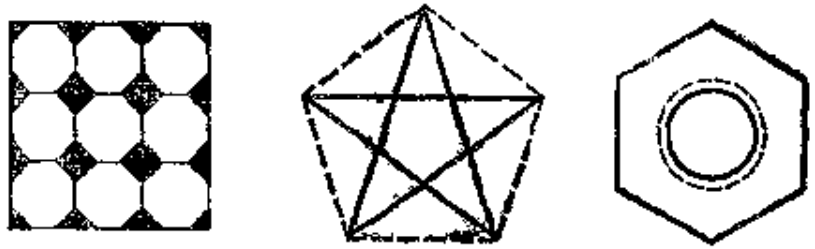
\includegraphics[width=7cm]{../pic/czjh2-ch7-63.png}
    \caption{}\label{fig:czjh2-7-63}
\end{figure}


正多边形和圆有非常密切的关系。
我们只要把一个圆分成几条相等的弧,就可以作出这个圆的内接或外切正 $n$ 边形。
下面我们来研究这个问题。

\begin{dingli}[定理]
    把圆分成 $n \; (n \geqslant 3)$ 等份:

    (1)依次连结各分点所得的多边形是这个圆的内接正 $n$ 边形;

    (2)经过各分点作圆的切线,以相邻切线的交点为顶点的多边形是这个圆的外切正 $n$ 边形。

\end{dingli}

我们以 $n = 5$ 的情况为例来进行证明。

已知: $\yuan\,O$ 中, $\yuanhu{AB} = \yuanhu{BC} = \yuanhu{CD} = \yuanhu{DE} = \yuanhu{EA}$,
$TP$、 $PQ$、$QR$、$RS$、$ST$ 分别是经过分点 $A$、$B$、$C$、$D$、$E$ 的 $\yuan\,O$ 的切线(图 \ref{fig:czjh2-7-64})。

求证:(1) 五边形 $ABCDE$ 是 $\yuan\,O$ 的内接正五边形;

(2) 五边形 $PQRST$ 是 $\yuan\,O$ 的外切正五边形。

\zhengming

(1) $\yuanhu{AB} = \yuanhu{BC} = \cdots = \yuanhu{EA}$

\quad $\tuichu \left\{\begin{aligned}
    AB = BC = \cdots = EA \\
    \yuanhu{BCE} = \yuanhu{CDA} = \cdots = \yuanhu{ABD} \quad \tuichu \quad \angle EAB = \angle ABC = \cdots = \angle DEA
\end{aligned}\right\}$

\quad $\tuichu$ 五边形 $ABCDE$ 是 $\yuan\,O$ 的内接正五边形。


(2) $\yuanhu{AB} = \yuanhu{BC} = \cdots = \yuanhu{EA}$

\quad $\tuichu \left\{\begin{aligned}
    AB = BC = \cdots = EA \\
    \angle PAB = \angle PBA = \angle QBC = \angle QCB = \cdots = \angle TEA = \angle TAE
\end{aligned}\right\}$

\quad $\tuichu$ $\triangle PAB$、$\triangle QBC$、 $\cdots$ $\triangle TEA$ 是全等的等腰三角形

\quad $\tuichu$ 五边形 $PQRST$ 是各边相等、各角相等

\quad $\tuichu$ 五边形 $PQRST$ 是 $\yuan\,O$ 的外切正五边形。

\begin{figure}[htbp]
    \centering
    \begin{minipage}[b]{7cm}
        \centering
        \begin{tikzpicture}
    \tkzDefPoints{0/0/O, 0/1.5/A}
    \tkzDrawCircle(O,A)
    \tkzDrawPoint(O)

    % 内接正五边形
    \tkzDefRegPolygon[center,sides=5,name=P](O,A)
    \tkzDrawPolygon(P1,P...,P5)
    \tkzLabelPoint[right](O){$O$}
    \tkzLabelPoint[above](P1){$A$}
    \tkzLabelPoint[left](P2){$B$}
    \tkzLabelPoint[left,  yshift=-.3em](P3){$C$}
    \tkzLabelPoint[right, yshift=-.3em](P4){$D$}
    \tkzLabelPoint[right](P5){$E$}

    % 外切正五边形
    \tkzDefLine[tangent at=P1](O)  \tkzGetPoint{p1}
    \tkzDefLine[tangent at=P2](O)  \tkzGetPoint{p2}
    \tkzInterLL(P1,p1)(P2,p2)  \tkzGetPoint{P}
    \tkzDefRegPolygon[center,sides=5,name=N](O,P)
    \tkzDrawPolygon(N1,N...,N5)
    \tkzLabelPoint[left](N1){$P$}
    \tkzLabelPoint[left](N2){$Q$}
    \tkzLabelPoint[below](N3){$R$}
    \tkzLabelPoint[right](N4){$S$}
    \tkzLabelPoint[right](N5){$T$}
\end{tikzpicture}


        \caption{}\label{fig:czjh2-7-64}
    \end{minipage}
    \qquad
    \begin{minipage}[b]{7.2cm}
        \centering
        \begin{tikzpicture}
    % 绘制已知的 正五边形
    \tkzDefPoints{0/0/A, 2/0/B}
    \tkzDefRegPolygon[side,sides=5,name=P](A,B)
    \tkzDrawPolygon[thick](P1,P...,P5)
    \coordinate (C) at (P3); % 后面还会用到这些点,所以将其命名为 C、D、E
    \coordinate (D) at (P4);
    \coordinate (E) at (P5);
    \tkzLabelPoint[left,  yshift=-.3em](A){$A$}
    \tkzLabelPoint[right, yshift=-.3em](B){$B$}
    \tkzLabelPoint[right](C){$C$}
    \tkzLabelPoint[above](D){$D$}
    \tkzLabelPoint[left](E){$E$}

    % 绘制外接圆
    \tkzDefLine[mediator](A,B)   \tkzGetPoints{a}{b}
    \tkzDefLine[mediator](C,D)  \tkzGetPoints{c}{d}
    \tkzInterLL(a,b)(c,d)  \tkzGetPoint{O}
    \tkzDrawCircle[very thick](O,A)
    \tkzLabelPoint[left](O){$O$}

    % 绘制内切圆
    \tkzDefPointBy[projection= onto A--B](O)  \tkzGetPoint{H}
    \tkzDrawCircle[very thick](O,H)

    % 其它
    \tkzDrawSegments[dashed](O,A  O,B  O,C  O,D)
    \extkzLabelAngel[0.5](C,B,O){$1$}
    \extkzLabelAngel[0.5](O,C,B){$2$}
    \extkzLabelAngel[0.7](O,B,A){$3$}
    \extkzLabelAngel[0.7](D,C,O){$4$}
\end{tikzpicture}


        \caption{}\label{fig:czjh2-7-65}
    \end{minipage}
\end{figure}

反过来,是不是每一个正多边形都有一个外接圆和一个内切圆呢?
我们仍以正五边形 $ABCDE$ 为例来研究这个问题。

经过顶点 $A$、$B$、$C$ 作 $\yuan\,O$, 连结 $OA$、$OB$、$OC$、$OD$ (图 \ref{fig:czjh2-7-65} )。

$\left.\begin{aligned}
    OB = OC \tuichu \angle 1 = \angle 2 \\
    \angle ABC = \angle BCD
\end{aligned}\right\}$

\qquad $\left.\begin{aligned}
    \tuichu \quad \angle 4 = \angle 3 \\
    OC = OB \\
    CD = BA
\end{aligned}\right\}$

\qquad $\tuichu \triangle ODC \quandeng \triangle OAB$

\qquad $\tuichu OD = OA \tuichu  $ 点 $D$ 在 $\yuan\,O$ 上。

同理,点 $E$ 在 $\yuan\,O$ 上。

所以正五边形 $ABCDE$ 有一个外接圆 $\yuan\,O$。

因为正多边形 $ABCDE$ 的各边都相等,所以它的外接圆的圆心 $O$ 到各边的距离都相等。
以 $O$ 为圆心,以这个距离为半径的圆和各边都相切。
所以,正五边形 $ABCDE$ 有一个内切圆。它的圆心就是外接圆的圆心。 于是得到:

\begin{dingli}[定理]
    任何正多边形都有一个外接圆和一个内切圆,这两个圆是同心圆。
\end{dingli}

正多边形的外接圆(或内切圆)的圆心叫做\zhongdian{正多边形的中心},
外接圆的半径叫做\zhongdian{正多边形的半径},
内切圆的半径叫做\zhongdian{正多边形的边心距}。
正多边形各边所对的外接圆的圆心角都相等。
正多边形每一边所对的外接圆的圆心角叫做\zhongdian{正多边形的中心角}。

\begin{figure}[htbp]
    \centering
    \begin{minipage}[b]{7cm}
        \centering
        \begin{tikzpicture}
    \pgfmathsetmacro{\R}{1.5}
    \pgfmathsetmacro{\n}{5} % 5 边形

    \tkzDefPoints{0/0/O}
    \tkzDefPoint(270:\R){A}
    \tkzDefRegPolygon[center,sides=\n,name=P](O,A)
    \tkzDrawPolygon(P1,P...,P\n)
    \foreach \i in {1,...,\n} {
        \tkzDrawLine[add=0.2 and 1.2](P\i,O)
    }
    \tkzLabelPoints[above, xshift=-.5em](O)
\end{tikzpicture}

% \begin{tikzpicture}
%     \tkzDefPoints{0/0/O, 0/-1.5/A}
%     \tkzDefRegPolygon[center,sides=5,name=P](O,A)
%     \tkzDrawPolygon(P1,P...,P5)
%     \foreach \i in {1,...,5} {
%         \tkzDrawLine[add=0.2 and 1.2](P\i,O)
%     }
%     \tkzLabelPoints[above, xshift=-.5em](O)
% \end{tikzpicture}


        \caption{}\label{fig:czjh2-7-66}
    \end{minipage}
    \qquad
    \begin{minipage}[b]{7cm}
        \centering
        \begin{tikzpicture}
    \pgfmathsetmacro{\R}{1.5}
    \pgfmathsetmacro{\n}{6} % 6 边形
    \pgfmathsetmacro{\halfn}{int(\n/2)} % 边数的一半。用于减少绘制时的重复动作。

    \tkzDefPoints{0/0/O}
    \tkzDefPoint(0:\R){A}
    \tkzDefRegPolygon[center,sides=\n,name=P](O,A)
    \tkzDrawPolygon(P1,P...,P\n)

    \tkzDefLine[mediator](P1,P2)   \tkzGetPoints{a}{b}
    \tkzDefLine[mediator](P3,P4)  \tkzGetPoints{c}{d}
    \tkzInterLL(a,b)(c,d)  \tkzGetPoint{O}
    \foreach \i in {1,...,\halfn} {
        \pgfmathsetmacro{\s}{int(\i + 1)}
        \tkzDefMidPoint(P\i,{P\s})  \tkzGetPoint{X}
        \tkzDrawLine[add=0.2  and 1.2](P\i,O)
        \tkzDrawLine[add=0.25 and 1.25](X,O)
    }
    \tkzLabelPoints[above, xshift=-.5em](O)
\end{tikzpicture}

% \begin{tikzpicture}
%     \tkzDefPoints{0/0/A, 1.6/0/B}
%     \tkzDefRegPolygon[side,sides=6,name=P](A,B)
%     \tkzDrawPolygon(P1,P...,P6)

%     \tkzDefLine[mediator](P1,P2)   \tkzGetPoints{a}{b}
%     \tkzDefLine[mediator](P3,P4)  \tkzGetPoints{c}{d}
%     \tkzInterLL(a,b)(c,d)  \tkzGetPoint{O}
%     \foreach \i in {1,...,3} {
%         \pgfmathsetmacro{\s}{int(\i + 1)}
%         \tkzDefMidPoint(P\i,{P\s})  \tkzGetPoint{X}
%         \tkzDrawLine[add=0.2  and 1.2](P\i,O)
%         \tkzDrawLine[add=0.25 and 1.25](X,O)
%     }
%     \tkzLabelPoints[above, xshift=-.5em](O)
% \end{tikzpicture}


        \caption{}\label{fig:czjh2-7-67}
    \end{minipage}
\end{figure}

正多边形都是轴对称图形, 一个正 $n$ 边形共有 $n$ 条对称轴,(为什么?)
每条对称轴都通过正 $n$ 边形的中心(图 \ref{fig:czjh2-7-66})。
如果正多边形有偶数条边,那么它又是中心对称图形,它的中心就是对称中心(图 \ref{fig:czjh2-7-67} )。

边数相同的正多边形相似。所以它们的周长的比等于它们的边长(或半径、边心距)的比,
它们的面积的比等于它们的边长(或半径、边心距)平方的比,


\begin{lianxi}

\xiaoti{(口答)矩形是正多边形吗?菱形是正多边形吗?为什么?}

\xiaoti{求证:}
\begin{xiaoxiaotis}

    \xxt{各边相等的圆内接多边形是正多边形;}

    \xxt{各角相等的圆外切多边形是正多边形。}

\end{xiaoxiaotis}


\begin{enhancedline}
\xiaoti{证明: 在正 $n$ 边形中,}
\begin{xiaoxiaotis}

    \xxt{中心角等于 $\dfrac{360^\circ}{n}$;}
    \xxt{中心角与外角相等。}

\end{xiaoxiaotis}

\xiaoti{(口答)一个正五边形,要绕它的中心至少转多少角度,才能和原来的正五边形重合?
    在不超过 $360^\circ$ 的范围内,这样的角度有几个? 正 $n$ 边形呢?
}
\end{enhancedline}

\end{lianxi}

